\section{Illustration of the system}
The reason for making a rich picture is to help one understand the interaction within a specific technology and/or product\cite{OOAD}. The drawing in Figure \vref{fig:Rig billede} is an overview of how the users (parents and kindergarten teachers) and the child would interact with the mobile device. Under the assumption that the multi-bachelor project \textit{GIRAF} has been implemented in everyday life, we want to show how it could be improved with an administrator program on the computer.

The mobile device is primarily used by the child as a communication tool by using using the application DigiPECS or aSchedule, but games can also installed to entertain the child. As a communication tool the child can ask for the user's help and the user can also use it to communicate with the child or tell the child to e.g. wash your hands before dinner. 
The users also need to use the mobile device when they want to add or edit something on the device e.g. schedule the next day's activities in aSchedule.  

 
The problem with the current \textit{GIRAF} system is that both the administrator and child need the same mobile device which could be at the same time. Some children will consider the mobile device theirs and therefore will not hand it over to the user or do so with much frustration. To resolve this problem without changing the mobile device primarily function, a computer program could be made, such that the user could administer the mobile device from a computer via some form of a wireless connection. This picture is shown in \vref{fig:Rig billede}. 

\begin{figure}[ht]
	\centering
		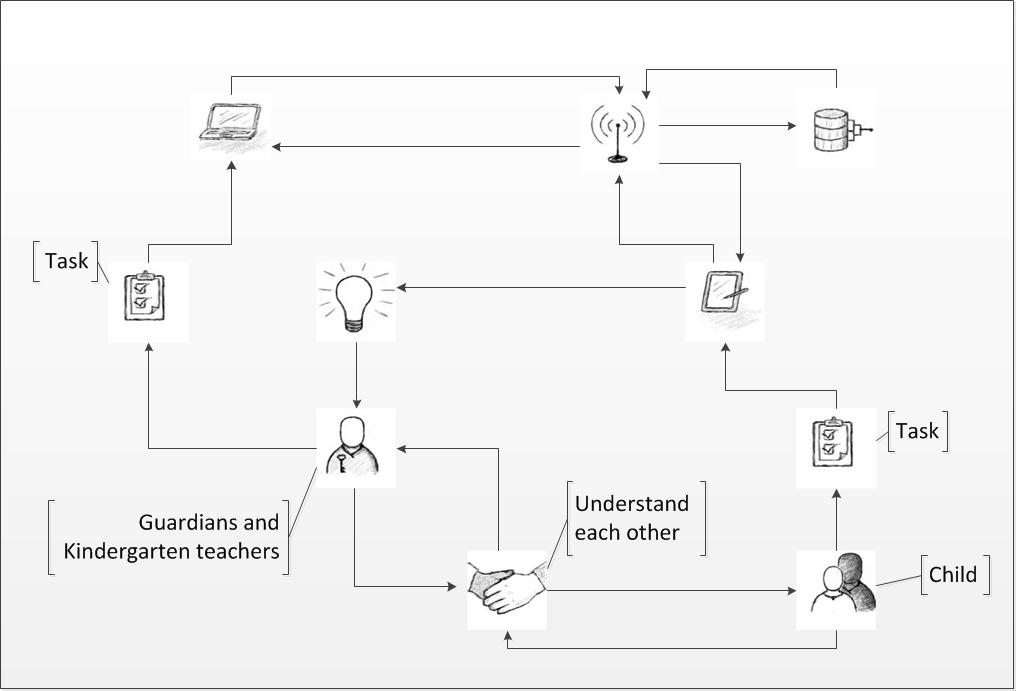
\includegraphics[width=1.00\textwidth]{img/Rig_billede2.jpg}
	\caption{The child uses the tablet to communicate with the parent or kindergarten teacher, such that the child and adult understand each other. The parent or kindergarten teacher uses a computer to administrate the tablet}
	\label{fig:Rig billede}
\end{figure}

In our project we want to make it possible to use a computer to change the mobile device setting, but our primary focus will be to make a digitized version of the contact book so that kindergarten teachers and parents, easily and quickly, can exchange information. The kindergarten teachers would then be able to write and send a summary of the child's activities including pictures of the involved activities to the parents. This is the base for our system definition.    